\documentclass{article}

% Language setting
% Replace `english' with e.g. `spanish' to change the document language
\usepackage[english]{babel}

% Set page size and margins
% Replace `letterpaper' with `a4paper' for UK/EU standard size
\usepackage[letterpaper,top=2cm,bottom=2cm,left=3cm,right=3cm,marginparwidth=1.75cm]{geometry}

% Useful packages
\usepackage{amsmath}
\usepackage{amsfonts}
\usepackage{graphicx}
\usepackage[colorlinks=true, allcolors=blue]{hyperref}
\usepackage{listings}

\usepackage{xcolor}
\newcommand\SC[1]{{\color{violet}{\it \bf Simon :} #1}}
\newcommand\ET[1]{{\color{red}{\it \bf Emile :} #1}}

\newtheorem{remark}{Remark}

\title{Project report : Probabilistic programming}
\author{Emile Trotignon and Simon Coumes}

\begin{document}
\maketitle

\section{Introduction}

For this project we have chosen to implement a probabilistic inference framework as a library in Ocaml.
This report takes most of the base knowledge about what we do in this project for granted.
We try with reasonable success not to repeat too much of your own lessons back to you.
Hopefuly nothing was made unclear as a result. \\

A few words about vocabulary.
In this document we consider separately the code that is actually written and executed and the ``corresponding probabilistic program''.
The later is the program whose set of executions define the distributions we build.
In generality we can consider that the user writes code that describes a probabilistic program.
This is done through the syntax we define.
An execution of said program is an assignment of a value to each variable that is ``sampled'' in the probabilistic program.
This defines a distribution on all possible outputs of the program (which the user can skew with statements such as $assume$ and $factor$). Our goal is to compute or approximate this distribution.

\section{Discrete inference by enumeration}

\subsection{Overview}

We build our language in Ocaml with a library that allow building probabilistic
programs (called models) as OCaml values representing ASTs, while still using
standard OCaml for control structures and alpha-reduction.

This means that although probabilistic constructs can be constructed dynamically,
control structures cannot.

We provide OCaml functions to build the AST that can be seen as syntactic sugar
for our probabilistic langage.

In this section, we restrain ourselves to discrete distributions with a finite
support and present our implementation of an inference method by exhaustive
enumeration. The use of an exhaustive enumeration of all possible executions is
made possible by the fact that all supports are finite.
All of this is found in the ``finite'' sub-library, and its associated
directory \texttt{lib/finite}.

\subsection{A recursive structure}

Our approach is centered on the introduction of a ``model'' type, which we inductively defined as follows :
\begin{equation}
	Model_1 ::= return \; e \; | \; (assume \; b), \; Model_2 \; | \; a = sample(d) \; in \;Model_2 \; | \;  (factor \; i), \; Model_2
	\label{eq:1}
\end{equation}

With $e$ an (OCaml) expression, $b$ an expression of type \texttt{bool}, $i$ an
expression of type \texttt{float}, $d$ an expression that has the type of a
distribution, and $a$ a variable name. We require in particular that every
expression be well formed with regard to free variables. ie all of their
free variables are bound either by normal Ocaml code or by a sample by the time they are encountered in
the tree this forms, and in general that they are valid OCaml expressions. \\

When we move to code, this gives the AST (Abstract Syntax Tree) from figure \ref{fig:AST1}.
\begin{figure}[h]
	\centering
	\begin{verbatim}
       type 'a t =
	  | Return : 'a -> 'a t
	  | Assume : (bool * 'a t) -> 'a t
	  | Factor : (Prob.t * 'a t) -> 'a t
	  | Sample : ('a Dist.t * ('a -> 'b t)) -> 'b t
    	\end{verbatim}
	% 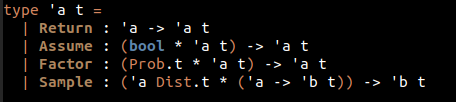
\includegraphics[scale=0.7]{images/AST1.png}
	\caption{Type definition for finite distributions}
	\label{fig:AST1}
\end{figure}

You may notice in \ref{fig:AST1} \texttt{Sample} constructor defines an existantial type, in
\texttt{\'a}.
This is because two models that represent a distribution with values of the
same type should have the same type, even if they sample distributions with
values of different types. This also means that any inference algorithm will
be unable to use the variable sampled, because they may have any type.

\SC{To reword : Note that the construction found in our models is existential.}


Perhaps more interesting, we can see how this can be used to define an example model (see figure \ref{fig:UglyEx}).
Please note that the bindings happening in samples in equation \ref{eq:1} are replace by functions here, which will be called during evaluation.
This approach will present multiples advantages and inconvenients in the rest of this project.

\begin{figure}[h]
	\centering
	\begin{verbatim}
let funny_bernoulli_ugly =
    Model.(
      Sample
        ( sample (Dist.bernoulli_int ~p:0.5)
        , fun a ->
            Sample
              ( sample (Dist.bernoulli_int ~p:0.5)
              , fun b ->
                  Sample
                    ( sample (Dist.bernoulli_int ~p:0.5)
                    , fun (c : int) ->
                        Assume (a = 1 || b = 1, Return (a + b + c))))))

	\end{verbatim}

	%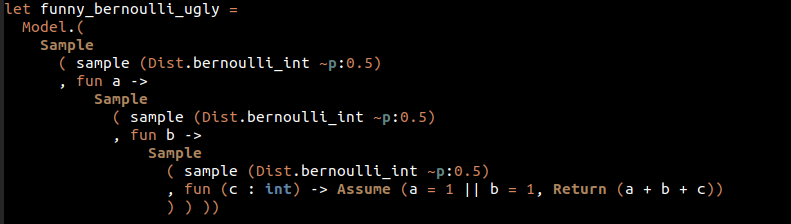
\includegraphics[scale=0.5]{images/ExampleUgly.png}
	\caption{A first code example with an unwieldy syntax}
	\label{fig:UglyEx}
\end{figure}

As shown in figure \ref{fig:UglyEx} this code is not very convenient to use. We will see in subsection \ref{subseq:sugar} how we used syntactic sugar to improve on this.

\subsection{Recursive evaluation}

We now want to perform a process of inference by exhaustive enumeration.
This means we want to look at each possible run of the probabilistic program our code describes and compute the corresponding score, avoiding all runs that fail an assume statement.
The result associated to a run is a pair $(value, score)$.

The recursive structure presented above allows this process to proceed recursively.
For each $sample$ statement, we can enumerate all possible outputs (each element of the support of the distribution we sample). For each possibility we bind the value to the corresponding variable and make a recursive call.
Each call gives us a list of results. We then output the concatenation of all those lists.

An $assume$ that evaluates to $true$ passes on the list of result we get by
evaluating its corresponding sub-model while an $assume$ that evaluate to false
returns the empty list (there are no corresponding executions).
\footnote{Remark that in the case of an $assume$ that returns false we do not
	explore the rest of the execution.}

Likewise, $factor$ statements pass on their values while changing the scores
and $return$ statement give a value together with the default score.

\begin{remark}
	For simple cases, this can be considered equivalent to looking at all
	possible results for each element in the cartesian product of the sets of
	possible results of all $sample$ statements in the code.
\end{remark}

\subsection{Syntactic sugar}
\label{subseq:sugar}

We introduced a let operator that allows one to sample distribution in a nicer
way.



\begin{figure}[h]
	\centering
	\begin{verbatim}
    Model.(
      let* a = Dist.bernoulli_int ~p:0.5 in
      let* b = Dist.bernoulli_int ~p:0.5 in
      let* c = Dist.bernoulli_int ~p:0.5 in
      assume (a = 1 || b = 1) (return (a + b + c)))
	\end{verbatim}
	\caption{A reformulation of the previous example with a better syntax}
	\label{fig:sugar}
\end{figure}

\section{Metropolis Hasting}

We now discuss the second method of inference we implemented, Metropolis Hasting.
This corresponds to the ``continuous'' sub-library of our implementation.

Like for the previous inference method we will not recall the general idea of
the method and will instead only describe the points of our specific approach
we consider the most relevant.

\subsection{Writing continuous distributions}

As we move to our second method of inference, Metropolis Hasting, we also start
to include continuous distributions. While a finite support distribution is
simple enough (a list of pairs of values and probabilities), we need a slightly
subtler representation for continuous distributions. For our purposes, they are
a pair of two functions. A function $sample$ allows to draw a value and a
function $logpdf$ which is the log of the probability density function of the
distribution.

From now on, when we speak of a distribution, we mean either a finite
distribution or a continuous one. Note that these can be mixed in the same code.
In concrete terms, this means we implemented a variant type in Ocaml with a
constructor for each case.

\subsection{A first execution}

The user has access to the same syntax as we presented in subsection
\ref{subseq:sugar}, the only difference being the kind of distribution allowed.
At first, we run the probabilistic program that this defines once. For each
probabilistic statement we encounter, we iteratively compute the
``current score'' of the run (more on how this is done in subsection
\ref{subseq:choice}). If the statement is a $sample$ we also store both the
current continuation and the current score for later (re)use. \\

When the execution is over this leaves us with a trace of the execution (all the
pairs of a continuation and a score that we computed) and with a final value and
score.

\begin{remark}
	Obtaining continuations is easy for us because the underlying structure of our
	code is still akin to the recursive definition we presented for the previous
	inference method. Hence, the ``continuations'' associated to a sample were
	already present in our approach to begin with.
\end{remark}

\subsection{Subsequent executions}

We now consider a hashtable that associates to each value we previously
encountered a single score. We choose at random a continuation, with a higher
probability to choose one of the older ones. Then we restart execution at this
point, taking the score we stored with this continuation as the current score.
All probabilistic statements following the corresponding point in the
probabilistic program are encountered anew (hence all random values after
this point are re-sampled). We also create a new list of pairs of computations
and scores, which differs from the previous one after the continuation with
which we started this new execution.

This creates a new trace.

We compare the score of this new trace with the previous one and choose which
one to keep.
The formula we use is that we keep the new trace with probability $\frac{W_{new}}{W_{old}}$.
With $W_{new}$ (resp $W_{old}$) the score of the new (resp old) trace. \\

If we kept the new trace we add the corresponding pair $(value, score)$ to the hashtable
\footnote{Please remark that our hashtable stores a list of scores associated to a value and not a single score.}
.
We then iterate this step with the trace we kept (which can be equal to the old one).

\subsection{Choices}
\label{subseq:choice}

The explanation above does not say :
\begin{itemize}
	\item How to iteratively compute the score of a trace.
	\item How to compute the final distribution using our hashtable.
\end{itemize}

The answer to the first question is that we multiply
\footnote{We do not store the log of the score to avoid rounding errors. This should be done in the future.}
the scores given by each probabilistic operator we encounter.
In the case of the $factor$ statement the associated score is straightforward.
Both the $observe$ and $assume$ statements can be seen as specific cases of factor.

This leaves us the $sample$ statement, which gives as a score the probability
associated by the sampled distribution to the value that was drawn. \\

In most cases the answer to the second question is easy.
If the hashtable contains no two entries with the same value we can output the
finite distribution that associates to each value the corresponding score.

However when there are duplicates we offer two options, neither of which give us exactly what we would like in all cases.
The first is to add the scores of all pairs that have the same value. This is
unwanted if there is a high chance of the code returning twice the same value
``in the same way''.
The second is to pick an arbitrary score.
The first is to add the scores of all pairs that have the same value. This is
unwanted if there is a high chance of the code returning twice the same value
by taking a different route.
Both option are left available to the user in our implementation. \\

\section{The tests}

We have implemented various tests and examples from the subject and class.
All these examples are available in the bin directory and can each be executed with the command ``dune exec bin/testname.exe'', with testname the name of the relevant test. \\

In no particular order :

\begin{itemize}
	\item ``coin'' implements the example seen in class where we guess the bias of a coin based on a series of tosses (assuming an uniform prior).
	\item ``laplace'' implements the example seen in class with the same name.
	\item Likewise for ``funny\_bernoulli''.
	\item ``risk'' implements the simulation of a round of the game Risk.
	      It is a bit unstable, because of the high number of samples involved.
\end{itemize}

\end{document}
